\chapter{Introduction} \label{chapter:intro}

\section{Motivation}

Uncertainty is an inherent component in clinical decision making. Despite our best efforts in biology, medicine, and pharmacology, significant gaps in our knowledge of the human body often lead to the adage that medicine is more an art than a science. 
% Parcelsus, "with the very processes of life, which must be understood before they may be guided

Several theories have been put forth regarding the medical reasoning process, including those of \citet{blois1984information} and \citet{paukerThresholdApproachClinical1980}. The majority of these theories propose clinical reasoning as a form of abductive, cyclical reasoning, establishing hypotheses given clinical evidence and then evaluating these hypotheses based on further testing. However, all wrestle with the underlying lack of complete information prior to a clinical decision. In this work, we conduct a series of decision-analytic experiments to investigate how the underlying uncertainty of a patient's state interacts with clinical cognition in an state-of-the-art \textit{in-silico} language modeling system: the large language model. 

Our experiments initially establish a theory of clinical uncertainty quantification in LLMs, before evaluating diagnostic decision making in increasingly complex scenarios. In Chapter~\ref{chapter:deprescribing}, we will evaluate LLM calibration under a complex, real-world clinical decision making task requiring expertise and gestalt. Following an investigation into uncertainty quantification, in Chapter~\ref{chapter:race-bayes} we further explore how our theory of clinical uncertainty influences Bayesian diagnostic reasoning in the LLM. We also see whether racial biases influence this Bayesian reasoning. Finally, in Chapter~\ref{chapter:bn-reasoning}, we extend the initial diagnostic reasoning task to a complete clinical evaluation scenario, framed as a sequential information seeking decision process.

\section{Paradigms in Clinical Cognition}
\label{subchapter:paradigms-clinical-cognition}
In order to frame the LLM as a clinical cognition experiment participant, we must first understand prevailing theories in clinical cognition in humans. There are currently two main paradigms that we will describe here. 

\subsection{The Problem-Solving Approach}

% Hypothetico-deductive framework
	% discuss the outcomes
% pushback against it because they didn't find any significant differences in expert and non-expert learners
% This led to work by Vimla on the forward reasoning process
% Later, Eva et al.37 showed that this was probably an epiphenomenon, con- founded with the use of post hoc probes and the observational nature of the data; it is not clear that success leads to forward reasoning on subsequent explanation of the case or forward reasoning leads to success
% This set the stage for the dual process theory
% How does this flow relate to the decision making literature? 

As a subset of human cognition, clinical cognition has often been investigated through cognitive science methods and principles. The first major investigations into physician information processing using cognitive science methods began with the seminal work of \citet{elstein1978medical} in their series of experiments, entitled the \emph{Medical Inquiry Project} research program. In it, they conduct a series of verbalization studies in which they have physicians evaluate standardized patient actors through a history of present illness and physical exam, the latter of which is conducted through conversations with a medical student acting as a "data bank". They then pause at regular intervals ("between the history and the physical examination" or "at the conclusion of the physical examination before ordering the laboratory tests")\citep{organizationStudyMedicalDiagnostic1970}.  to reflect and summarize their current problem solving processes. Similar work at McMaster University was conducted that instead used a method of "stimulated recall" to encourage reflection by playing back physician-simulated patient interactions. The goal in both programs was to identify a generalized cognitive framework of expert clinical decision making. Given this hypothesis, the authors limited the breadth and depth of their studies significantly. Namely, the number of cases and the number and type of physicians were both limited, under the assumption that a general expert physician (defined not by their relevance to the clinical case at hand, but by peer-rated excellence scores) should be able to demonstrate the general cognitive problem solving process. Perhaps as a result of these limitations, the authors of the Medical Inquiry Project found that there was no objective difference in diagnostic accuracy between experts and non-experts. They further found that expertise was context-dependent and good performance on one case did not predict good performance on another, further suggesting that a single problem solving framework was unlikely and clinical knowledge influenced in expert problem solving. 

While they were unable to determine the cognitive framework that differentiated effective diagnosis, they identified that all physicians followed a \emph{Hypothetico-deductive reasoning} process. This cognitive framework described a process by which physicians generated a limited set of hypotheses (4 $\pm$ 1) early in the exam and used them to guide further data collection. While the hypothetico-deductive reasoning model has had far-reaching impacts on clinical cognition, diagnostic AI, and medical education to this day, due to the limited number of clinical cases evaluated, it could not be concluded to be the cognitive problem solving process of expert physicians, as physicians that both arrived at the correct diagnosis and those that did not, seemed to employ it. This gap led to a flurry of subsequent work attempting to explain the difference in cognitive processes in clinical problem solving. 

One hypothesis (later supported by one of the authors of MIP itself \citep{elsteinThinkingDiagnosticThinking2009}) was that expertise in a given clinical situation played a key role in determining the type of cognitive process employed. For example, \citep{groenMedicalProblemsolvingQuestionable1985}, among others, find that physicians in a familiar situation (i.e. one where they have strong expertise) do not display explicit hypothesis testing \citep{schmidtCognitivePerspectiveMedical1990, brooksRoleSpecificSimilarity1991, evaExploringEtiologyContent1998}. They named this process the \emph{forward reasoning} process, compared to the \emph{backward reasoning} of the hypothetico-deductive framework. They further identified that subexpert cardiologists that arrived at the incorrect diagnosis performed a hybrid process of forward and backward reasoning, rather than simply forward reasoning. They conclude that experts begin their reasoning process in their knowledge base, rather than by developing hypotheses. Further evaluation of the knowledge structure itself determined that expert diagnosticians have learned a diverse and abstracted network of semantic relations between clinical findings and potential diagnoses \citep{bordageSemanticStructuresDiagnostic1991, patelKnowledgeBasedSolution1986}. However, forward, intuitive, and rapid reasoning is not the only necessary reasoning strategy. In fact, later, \citet{patelMedicalExpertiseFunction1990} found that forward reasoning breaks down under complexity and uncertainty. The relative and joint benefits of both the  hypothesis testing and data-driven, forward reasoning would lead some to advocate for a cognitive dual reasoning strategy model \citep{evaHeuristicsBiasesBiased2005}. A decision making theory borne from psychology discussed in the next section seems to bridge the gap.  

% This work  also inspired the seminal work on information processing by \citet{simonHumanProblemSolving1971}, in which they describe problem-solving as a search through an operator space from an \emph{initial state} to a \emph{goal state}. 

\subsection{Dual Process Theory: A Theory of Decision-Making}
% Dual process theory is borne out of the psychologist's decision making literature, particularly under uncertainty. 
% It was quickly adopted by clinicians (point to Pat Croskerry) and comfortably integrates some of the tension between Vimla's work on expertise/forward reasoning and the original hypothetico-deductive framework. It seems to be modulated by a number of charactersistics, one of which (relevant to our work) is uncertainty, but also expertise. 

The prevailing theory of general cognitive decision making today is known as \emph{dual process theory}, originally proposed by \citet{shiffrinControlledAutomaticHuman1977} as a "two-process theory of human information processing". It has since gone through several iterations, being popularized in cognitive psychology by the work of Hammond and colleagues \citep{epsteinIntegrationCognitivePsychodynamic1994, hammondHumanJudgementSocial1996}, and in the general public by Kahneman \citep{kahneman2011thinking}. The two systems have since been dubbed System 1 and System 2, to be described later. 

However, the origin of these cognitive systems comes from early decision making literature relying on normative models of decision making. The decision-making approach to cognition forgoes protocol methods eliciting cognitive processes from experts and assumes a normative model of decision making that expert and subexpert physicians should adhere to, often based on a Bayesian or utility-based model. The first work in this space established a two stage clinical reasoning model based on aligning symptom complexes with disease complexes. In the first stage, a set of potential diagnoses are identified based on patient symptoms. In the second, a decision-analytic approach is taken to determine the conditional likelihood of a disease, given a symptom complex and lab tests. This process is iterated upon until the final diagnosis is reached \citep{ledley1959reasoning}. However, work in cognitive science led to the realization that more could be learned from investigating the cognitive processes of experts, rather than prescribing an optimal decision making process through some optimization function \citep{patelEmergingParadigmsCognition2002}, as there are a number of other considerations that a rational choice theory does not take into account. Thus began the aforementioned problem-solving research paradigm. 

Despite this initial reticence, there was some limited work on integrating a probabilistic approach with clinical cognition \citep{blois1984information}. Some relied on Bayes' theorem to develop a framework of updating disease estimates following the acquisition of new information \citep{huninkDecisionMakingHealth2014, soxMedicalDecisionMaking2013, paukerThresholdApproachClinical1980}. We leverage this paradigm in Sections~\ref{chapter:race-bayes} and \ref{chapter:bn-reasoning}. Much of the work in System 1 and 2 thinking arises from attempting to understand predictable errors in probabilistic judgement \citep{tverskyFramingDecisionsPsychology1981} which in the clinical space has been called \emph{cognitive dispositions to respond} \citep{croskerryImportanceCognitiveErrors2003}. These led to a set of \emph{heuristics} that simplify decision making under uncertainty \citep{tverskyJudgmentUncertaintyHeuristics1974}. The existence of such heuristics in the clinical domain was quickly theorized \citep{eddyProbabilisticReasoningClinical1982}. However, heuristics are prone to biases that may lead to the incorrect conclusion, including anchoring \citep{friedlanderAnchoringPublicityEffects1983}, confirmation bias \citep{klaymanDebiasEnvironmentInstead1993}, and framing effects \citep{mcneilElicitationPreferencesAlternative1982}. Therefore, it was theorized that two different cognitive processes are employed interchangeably based on the cognitive task at hand. Namely, to use Kahneman's parlance, System 1 and System 2 Thinking, as described in further detail below:

\begin{enumerate}
    \item \textbf{System 1:} A cognitive system described as "intuitive" and "experiential". It is largely a automatic, reflexive system used to make decisions rapidly with minimal cognitive load. It uses information immediately available, while sometimes limited, to make a holistic judgement. These decisions are often governed by habit and are difficult to control or intervene upon.
    \item \textbf{System 2:} A more deliberate cognitive system, used for more methodical and "rational" or "analytical" decision making. This system utilizes additional information actively collected by the individual from their environment. Decisions are made by applying a set of learned rules consciously. Decision making is also actively monitored and metacognitive steps such as doubt are governed by System 2 \citep{epsteinIntegrationCognitivePsychodynamic1994, hogarthEducatingIntuition2010,  kahnemanPerspectiveJudgmentChoice2003}.
\end{enumerate}
     

This new cognitive decision making paradigm was quickly adopted by clinicians and comfortably reconciles \citet{patelKnowledgeBasedSolution1986}'s work on data-driven, forward reasoning and the original hypothetico-deductive framework. In the clinical domain, System 1 is often referred to as clinical gestalt or a "gut feeling" and is often dependent on the pathognomicity of the presentation \citep{croskerryUniversalModelDiagnostic2009}. Recognizing patterns of clinical features and diagnoses is a function of System 1 thinking \citep{groenMedicalProblemsolvingQuestionable1985, blois1984information}. Conversely, System 2 thinking in the clinical domain is characterized by a slower, more taxing, analytical decision making process. This may be triggered in a physician when the presentation is unrecognized or ambiguous. System 2 can also override an initial System 1 judgement if there are clinical features that do not indicate an initial, reflexive diagnosis.

The decision on which System to use however, is interesting and modulated by a variety of criteria. Recent work shows that System 2 thinking subjugates System 1 processing when the situation is complex or ill-defined, the stakes are high, or in the context of uncertainty \citep{croskerryCriticalThinkingReasoning, moultonSlowingWhenYou2007}. In this thesis, we are chiefly concerned with uncertainty. We believe that in such a setting, System 2 thinking should be employed and therefore, we consider a normative, decision-making approach leaning on probabilistic reasoning. We encourage the LLM to reason deliberately and analytically given the ambiguity of the clinical contexts we present it with. In addition to this theoretical frame, there are a number of practical reasons for choosing the decision-making paradigm, rather than the problem-solving one described earlier. We will enumerate these below. 


% Studies in the lab have also experimentally validated the existence of a number of biases that arise from such heuristics, Much of this work is validated using a normative frame, in which either expected utility or Bayesian-optimal function is used to determine the "ideal" state \citep{camererProcessperformanceParadoxExpert1991}. 


\subsection{Benefits of the Normative Approach}
Both the problem-solving and decision-making cognitive theories offer productive lenses through which to view a clinical cognitive study of large language models. As mentioned, both are rooted in rigorous cognitive research that demonstrate their ability to model physician diagnostic decision making in a variety of clinical contexts. Furthermore, both have been used as inspiration for clinical AI systems, and therefore demonstrate their usefulness in developing computational models of cognition \citep{clanceyNEOMYCINReconfiguringRulebased1981, gronchiDualprocessTheoriesThought2024}. Lastly, we could employ both frames to design a set of experiments to evaluate the LLM as a subject in a clinical cognitive psychology experiment \citep{binz2023using}. For instance, we could present cases to the LLM, as has been done in the past and evaluate its error modes \citep{kanjee2023accuracy}, assuming that it has some clinical expertise and describe its cognitive processing as one would in the problem-solving paradigm. Conversely, we could present these same cases to the LLM and assume a normative approach that should be taken through a decision-making frame. Here, we will argue why we take this latter approach. 

As the LLM will ultimately be used as a collaborative tool in clinical decision making, it is important to validate its accuracy, as well as its cognitive processes. Using a descriptive, information-processing approach, we are limited to describing and classifying its cognitive process, but aren't able to ground its responses in an objective answer. Using our normative, decision-analytic frame, we are able to evaluate LLM reasoning against a ground truth. Several normative functions have been proposed in the decision making literature, including expected utility \citep{briggsNormativeTheoriesRational2023} and Bayesian models \citep{maBayesianDecisionModels2019}. We elect to use a Bayesian frame, as we are chiefly interested in patient outcomes, not cost-effectiveness or other metrics of optimal decision making strategy, as is common to utility functions. 

However, in our consideration of Bayesian decision making, we must reconcile several well founded critiques of the decision-making approach by it's descriptive opponents. The first of which is well-founded that humans are not Bayesian thinkers \citep{gigerenzerToolsTheoriesHeuristic1991}, and therefore we cannot use a Bayesian grounding for the normative state. While this may be true for humans, we argue that it isn't true for LLMs, as demonstrated in our work in Section~\ref{chapter:race-bayes} as well as by others \cite{nafarProbabilisticReasoningGenerative2024b}. We see that LLMs are capable of engaging in reasoning that aligns explicitly with Bayesian principles. However, whether a Bayesian function provides the \emph{optimal} decision function in a clinical scenario is more difficult to examine. In this work, we select Bayesian information utility as a reasonable choice, but it could be easily replaced by others in our evaluation framework. We also agree with proponents of the information-processing approach who maintain that the biases or "fallacies" identified by normative approaches may in fact be a function of irrational, but otherwise meaningful, components of clinical care (e.g. patient requests, cost considerations, etc.). However, these heuristics must be developed as a function of expertise \cite{patel1991general}. Namely, expert physicians working in their area of expertise, often employ heuristics such as confirmation bias successfully, as compared to subexperts \cite{patelEmergingParadigmsCognition2002}. We view the LLM as a subexpert clinical decision maker for several reasons. As shown in a variety of work \cite{rydzewski2024comparative}, while state-of-the-art LLMs perform well on some tasks, they are still far from expert clinical reasoners \cite{harrisLargeLanguageModels2023}. Therefore, we believe that we can use a more decision-analytic framework to evaluate them, rather than assume that their biases are a function of expertise, and therefore valid decision making practice.

Finally, while we are largely leveraging a normative evaluation framework, we are not solely concerned about the final diagnostic decision. As \citet{patelEmergingParadigmsCognition2002} puts it, a key difference between the two cognitive paradigms is that "Problem-solving research emphasizes the sequential process of searching for a solution path, whereas decision research focuses more on the nature of the decision outcome and how it may deviate from an acceptable normative standard." However, in Section~\ref{chapter:bn-reasoning}, we forgo this assumption of decision-making theory and evaluate sequential Bayesian decision making. We will leverage the LLM's unique ability to explicate its reasoning as it performs decision-making to both evaluate the decision-making process, as well as the final decision itself. Given the aforementioned advantages, we believe that leveraging a decision-making cognitive framework with a Bayesian utility function will yield unique insight into an LLM's cognitive process. 

 
\section{LLMs as Candidate Models of Clinical Sublanguage Processing}
In the previous section (\ref{subchapter:paradigms-clinical-cognition}), we discussed the cognitive decision making frame that we would be borrowing from in our clinical cognitive evaluation of LLMs. As our chief modality of study is language, a product of large language models, in this section, we will argue why this product is worthy of study, how it relates to the clinical sublanguage, and why LLMs potentially present a unique linguistic theory of the clinical sublanguage. To begin, we provide a brief overview of Zellig Harris' theory of sublanguages. For our purposes, this will provide background for a view of the clinical sublanguage, so far as it has been constructed. Moreover, it will allow us to view the large language model as a novel, generative theory on the clinical sublanguage. This motivates our use of it in a cognitive study of uncertainty. 

\subsection{Harris' Sublanguage Theory}
Zellig Harris (1909-1992) was an instrumental linguist, semiotician, and "methodologist" \cite{nevinZelligHarrisAppreciation} that significantly influenced 20th century American linguistics. His \emph{distributional hypothesis}, despite being misconstrued, has largely motivated much of the past few decades of research in computational linguistics. Namely, embedding models from word2vec through present-day LLMs are based on an idea of distributional semantics that was first derived from Harris' work. As we will discuss later, the original distributional hypothesis was pertaining co-occurrences of word classes and their relative positions to one another in sentence structures. It was therefore a method of formal characterization of the structure of language. Harris' explicitly states that there is no one-to-one map between the distribution of word classes and meaning, a point that has been largely ignored by current NLP researchers. 

Harris made another significant contribution to formal semantic theory with his work on sublanguages. Harris defines a sublanguage as "subsets of sentences that are closed under certain operators in a language" \cite{harrisTheoryLanguageInformation1991}. Put simply, a grammatical operation carried out on any sentence in the sublanguage yields another sentence in the sublanguage. Sublanguages have certain properties that distinguish them from other constructs of language variation, namely, registers and dialects. Registers and dialects are both variations of language restriction that arises from different sociolinguistic contexts and use cases. Specifically, both have either specific operators or language features that are either included or excluded from the general language. Registers in particular are used for a particular function, such as newspaper headlines and recipes \cite{zwickyChapterRegisterDimension2015}. Despite their similarity in being a restricted subset of a language, they differ significantly from sublanguages. Mathematically, a sublanguage can be defined by the existence of a metalanguage that describes the sublanguage grammar. The sublanguage grammar can be described by a set of word-classes and the grammatical operators that exist between them. We can make this definition more tangible through an examination of Harris' seminal work on the immunology sublanguage, which just happens to relate somewhat to the clinical sublanguage central to our work. 

Harris used his theory of sublanguage to investigate a particular subfield of early immunology: the search for the cell that produces antibodies conducted from 1940-65. Together with colleagues, he lays out a complete grammar describing this corpus by collecting words into classes by co-occurrence and defining a closed set of world-class sequences (sentence structures).  Instead, we will just describe a few key structures that shed light on the way that sublanguages are defined. The first sentence structure Harris defines is using 3 word classes. Namely, he identifies class $\mathbf{A}$ as a subject of \emph{found in the lymph nodes after injection of an antigen}, a verb of class $\mathbf{V}$ that consists of \emph{is found in, is contained in, is produced by}, and an object class $\mathbf{T}$ consisting of nouns such as \emph{lymph nodes, lymph, serum}. These create a sentence structure of $\mathbf{AVT}$ to create sentences such as \emph{Antibodies are produced by lymph nodes} or transformed as \emph{Lymph nodes produce antibodies} \cite{harris2012form}. Harris further argued that precisely defining a sublanguage grammar is one way of converting language into information. Namely, he describes methods of weighing the relative evidence of claims in various papers in the corpus through the occurrence of certain sentence structures. This second-order analysis is outside the scope of this thesis, except to point out that we can derive additional information by describing a subfield through a sublanguage. 
% While this work was an impressive effort in standardizing the language of science, a full review of it is outside of the scope of this thesis.
\subsection{What makes a complete sublanguage?}
\begin{figure}
	\centering
	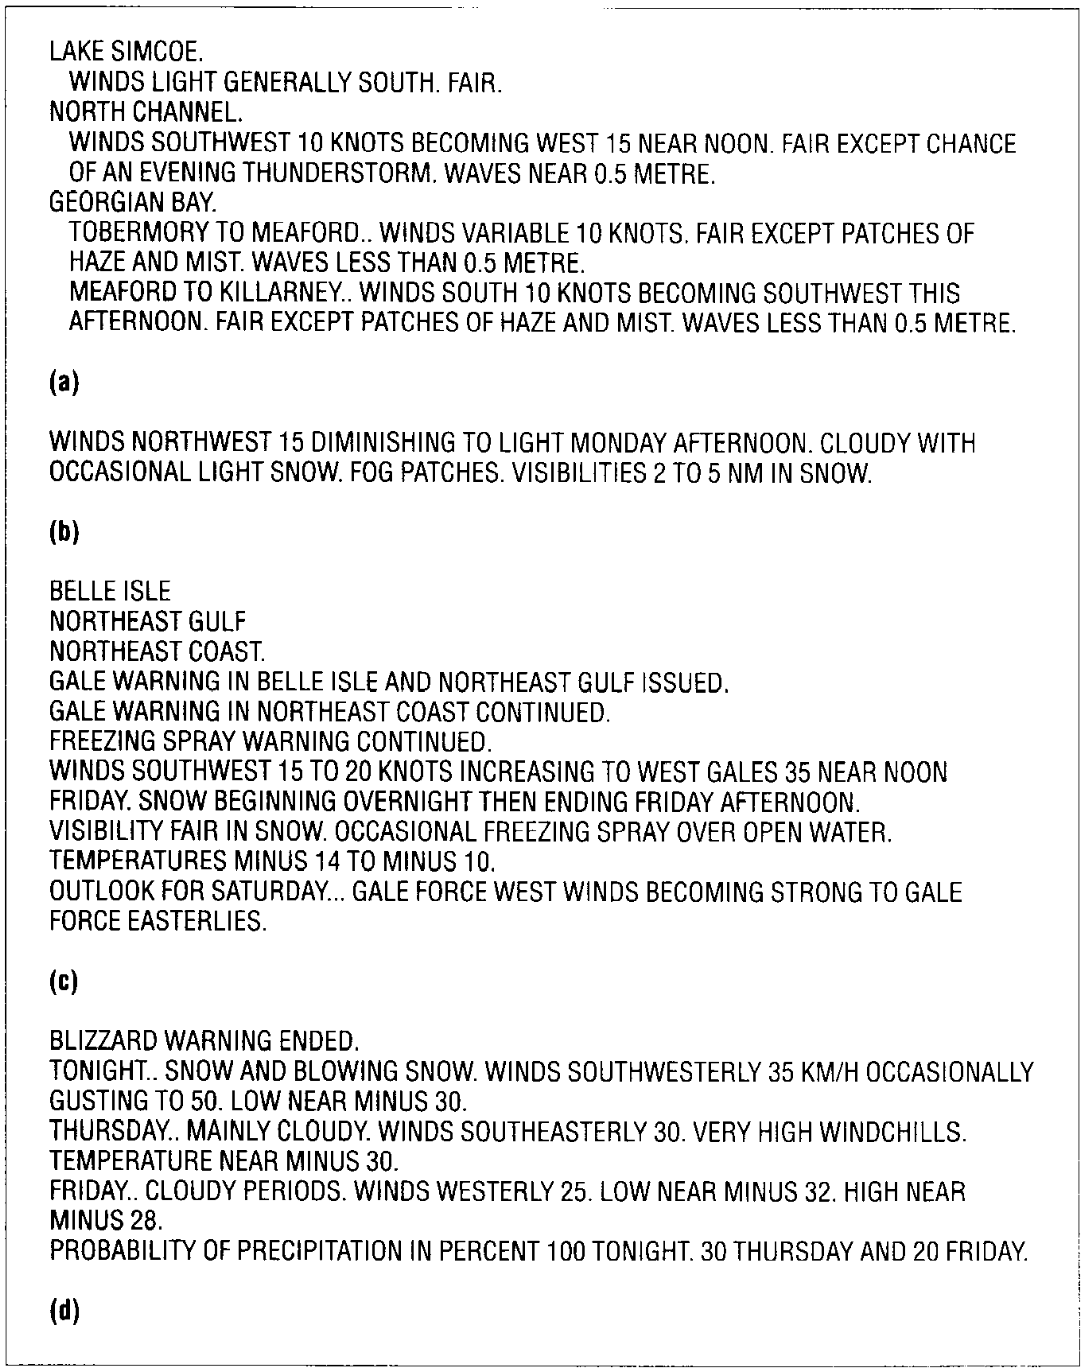
\includegraphics[scale=0.40] {figures/fog_text_message.png}
	\caption{Forecast text messages by region: (a) Great lakes marine; (b) Arctic marine; (c) Atlantic marine; (d) public \emph{reproduced from \cite{goldbergUsingNaturallanguageProcessing1994}}} \label{fig:fog-text}
\end{figure}

Despite the considerable work put into the definition of the immunological sublanguage by Harris, he notes that further articles need to be analyzed in order to describe certain meta-science segments and grammatical structures such as quantifiers and sentences with conjunctions. We claim that he clinical sublanguage is poorly defined and fuzzy. In order to validate this claim, we first describe a complete and well-formed sublanguage used in one of the first natural language generation systems: the forecast generator (FoG), used to generate computer-readable forecasts from short-form narratives describing the results of weather simulations in both English and French \citep{goldbergUsingNaturallanguageProcessing1994}. The reports were disseminated as text messages and following a distinctive telegraphic style sublanguage, as shown in Figure \ref{fig:fog-text}. An initial distributional analysis of the million-word corpus led to the definition of a Backus Naur Form (BNF) grammar and distribution of a lexicon and syntactic structures found in forecasts. Combined with a state-of-the-art generative theory at the time (based on Meaning-Text Theory from Igor Mel'čuk and Aleksandr Zholkovsky \citep{ivanovaMeaningTextTheory2022}), they were able to deploy their NLG algorithm throughout the Canadian weather service across several forecast types. They found that adding new forecast types within the sublanguage required very little change to the sublanguage, reasonably validating their generated grammar. Further evidence came from the adaptation of the grammar to neatly accommodate language "drift" as forecaster language evolved \citep{kittredgeSublanguageEngineeringFoG1994}. Their sublanguage grammar was largely robust against modification despite new documents that should still exist within the sublanguage, thereby demonstrating a closed grammar.

\subsection{The limitations of the current clinical sublanguage}
Having seen the robust grammar of the FoG system, we can contrast it against that of the clinical sublanguage as defined by \citet{friedmanTwoBiomedicalSublanguages2002}. The authors explicitly state that this sublanguage is developed for patient reports. The work conducted on the clinical sublanguage was based on two prior NLP systems: the Linguistic String Project \cite{sagerNaturalLanguageProcessing1994} and the MedLEE system \cite{friedmanGeneralNaturallanguageText1994}, both of which used a constituent grammar formalism compared to the operator-argument formalism proposed in Harris' work. The MedLEE grammar, initially developed for the chest radiology report sublanguage, has been extended to include discharge summaries, pathology reports \cite{friedmanBroadcoverageNaturalLanguage2000}, and nursing narratives \citep{hyunExploringAbilityNatural2009}. Despite its impressive versatility with limited changes to the underlying grammar, both the authors \cite{lussierAutomatingSNOMEDCoding2001} and others \cite{sevensterAutomaticallyCorrelatingClinical2012} have found that its parsing was not perfect. Namely, MedLEE incorrectly categorized word classes, such as misunderstanding T1 and T2 as the 1st and 2nd thoracic vertebrae instead of T1 and T2 relaxography (MRI protocols). It also struggled with multiple modifiers of body locations (\emph{upper inner quadrant of the left breast}), despite them being added to the vocabulary, indicating that the underlying grammar was not complete \cite{lussierAutomatingSNOMEDCoding2001, jainIdentificationSuspectedTuberculosis1996}. However, the main limitation of the MedLEE system comes from its sentence-by-sentence processing, leading to poor anaphora resolution. While sublanguage grammars conventionally consist of word classes and sentence-structures, in discourse settings, they result in discourse word classes and between-sentence structures. Such a construction would be necessary to effectively resolve the grammar proposed in MedLEE. However, the inclusion of discourse parsing would significantly complicate the grammar and could potentially make its ruleset excessively complex, though this remains to be tested. Based on this analysis of the current state of the clinical sublanguage, we conclude that further work needs to be done in establishing the grammatical rules of such a sublanguage. To that end, we propose that current distributional semantic models can act as such a bridge.

\subsection{Introduction to Distributional Semantic Models}
Before we can describe how an LLM might act as a candidate model for clinical sublanguage processing, an introduction to the transition from Harris' original sublanguage theory to distributional semantic language models is necessary. The underlying hypothesis in Harris' distributional theory was that we can describe a language as the co-occurrences of its parts in relation to one another, irrespective of history or meaning, and words can be fully specified by the sum of all the environments that they appear in \citep{harrisDistributionalStructure1954a}. As discussed, he explicitly denies the claim that there is a one-to-one relationship between these occurrences and meaning. However, in practice, this simplification has proved useful, often described succinctly as "a word is characterized by the company it keeps" \citep{firth1957synopsis}. This adage has led to distributional semantic models that lay the foundation for the modern day Large Language Model (LLM). Given that LLMs are neural network-based models, we will mostly focus on models following the development of dense, continuous word representations such as word2vec. Prior to these models, dimensionality reduction \citep{sahlgren2005introduction, landauerSolutionPlatosProblem1997} or matrix decomposition \citep{baroni2010distributional} methods over word co-occurrence matrices were common. 


\begin{wrapfigure}{r}{0.70\textwidth}
    \begin{center}
        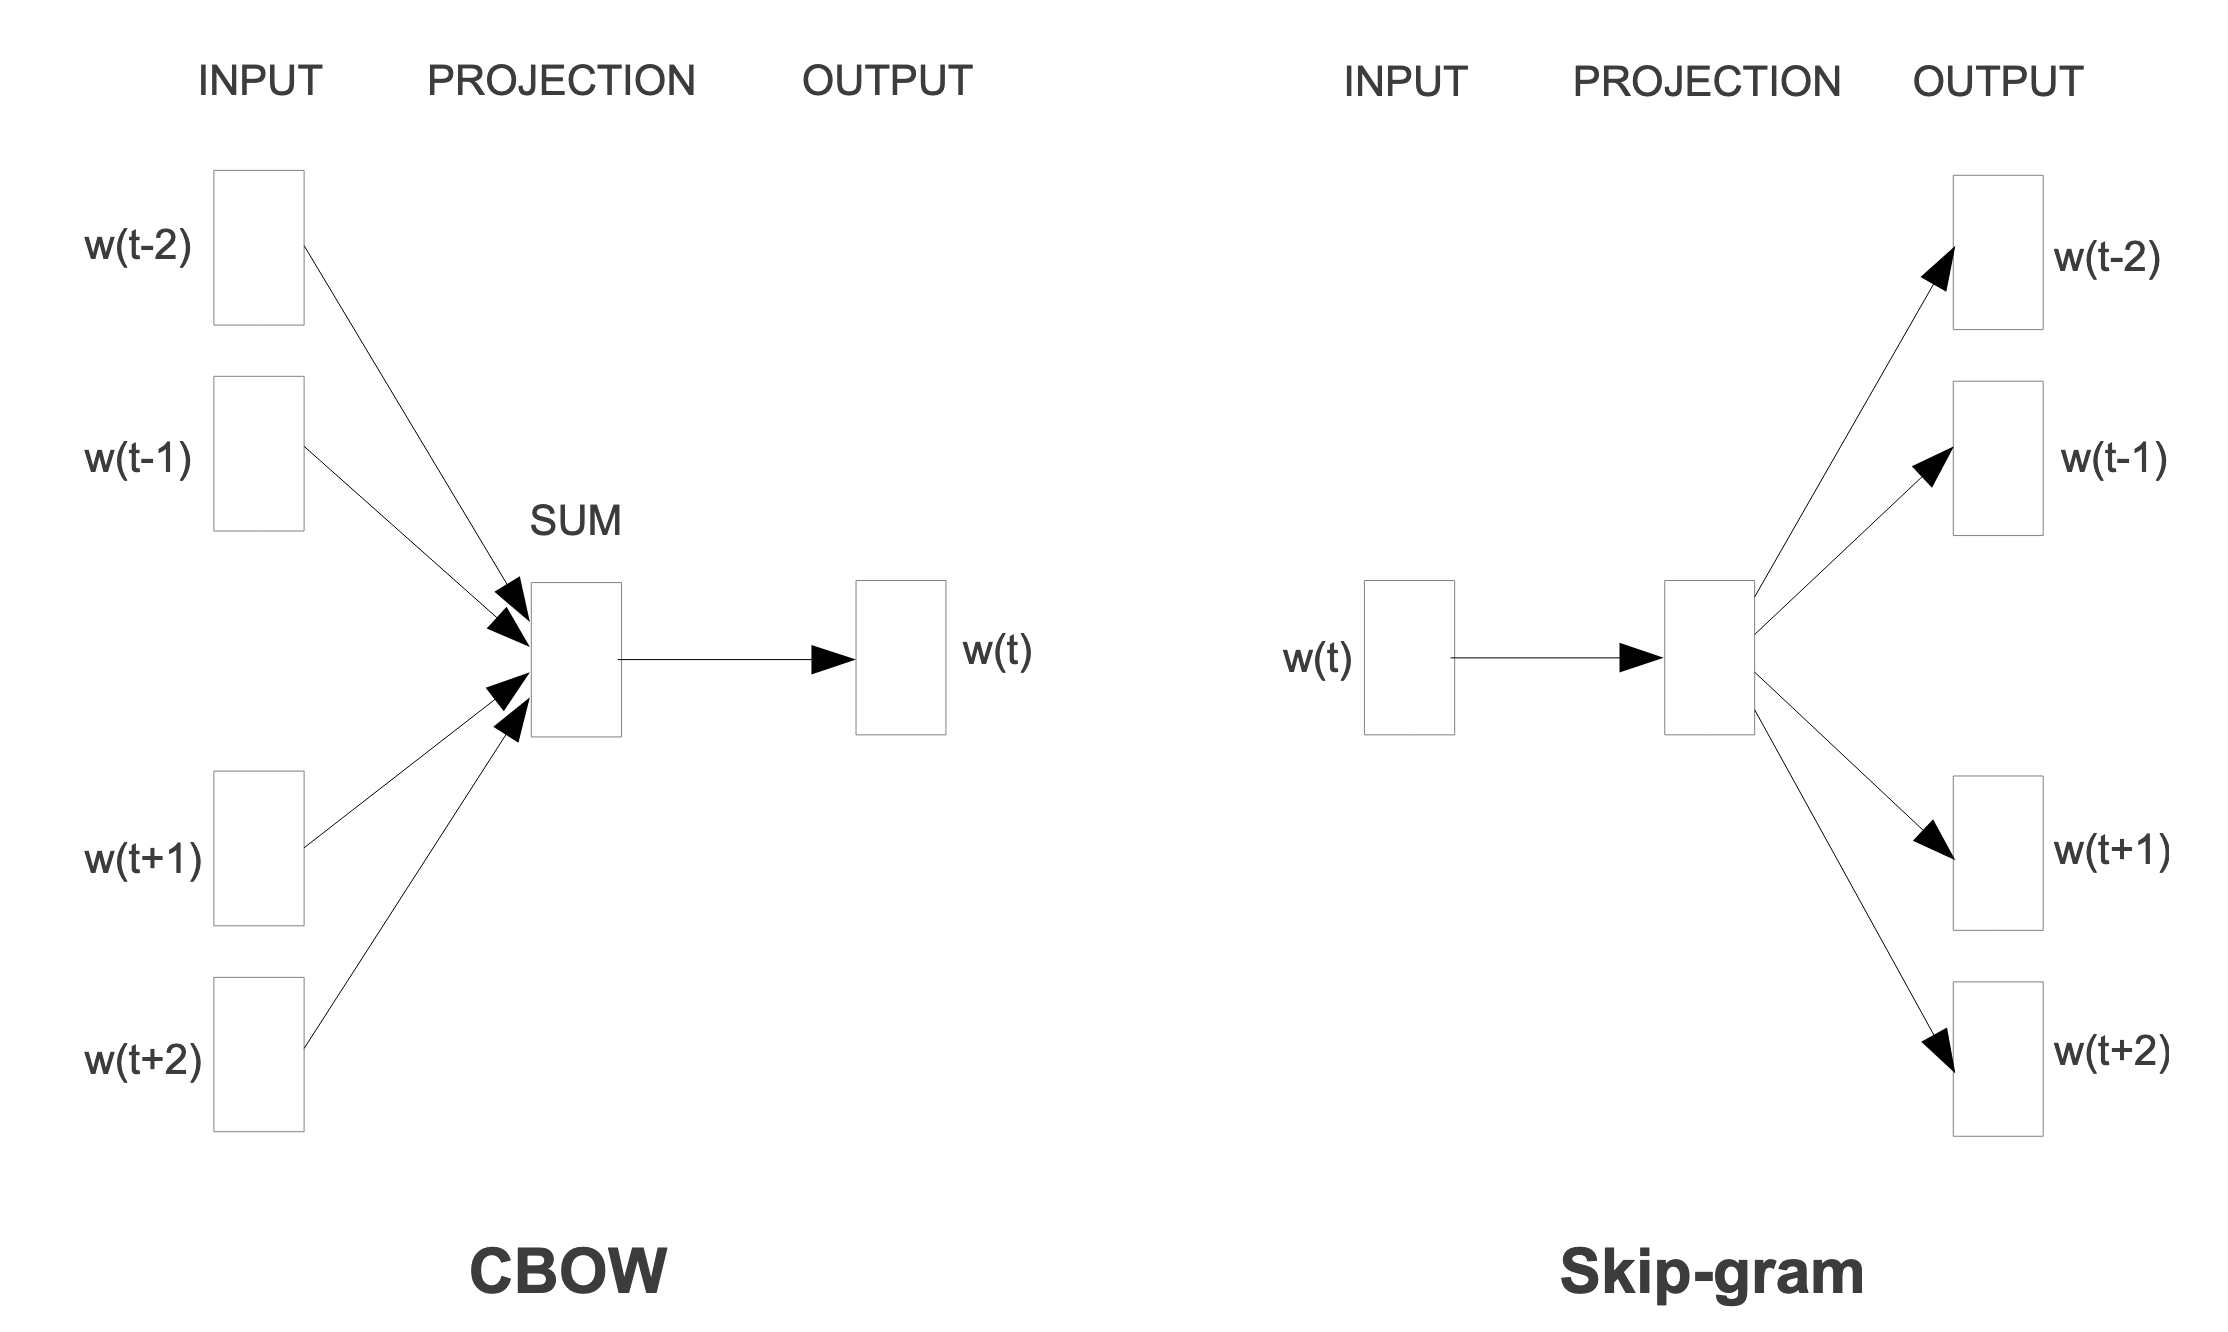
\includegraphics[scale=0.25] {figures/word2vec_architectures.png}
        \caption{ Architectures of the word2vec models \emph{reproduced from \cite{mikolov2013efficient}}}
    \label{fig:word2vec}        
    \end{center}
\end{wrapfigure}

Instead of first learning computationally-expensive co-occurrence matrices, word2vec models directly draw from Harris' theory by using learning word representations using a context window of surrounding words. The continuous bag-of-words (CBOW) model is trained using a "fill-in-the-blank" approach, where a fixed length representation of a word, known as its embedding, captures the likelihood of other words appearing within the context window, as shown in Figure~\ref{fig:word2vec}. Words that have similar meanings are expected to impact these probabilities in similar ways, since they tend to occur in similar contexts. Similarly, the continuous skip-gram model trains word embeddings by predicting the words in the context window from a single word. Both models were trained with classic neural network loss functions and optimizers, namely cross-entropy loss and stochastic gradient descent, respectively. \citet{mikolov2013efficient} found that the CBOW model trains faster while the skip-gram performs better with infrequent words. 

\begin{figure}[htbp]
	\centering
	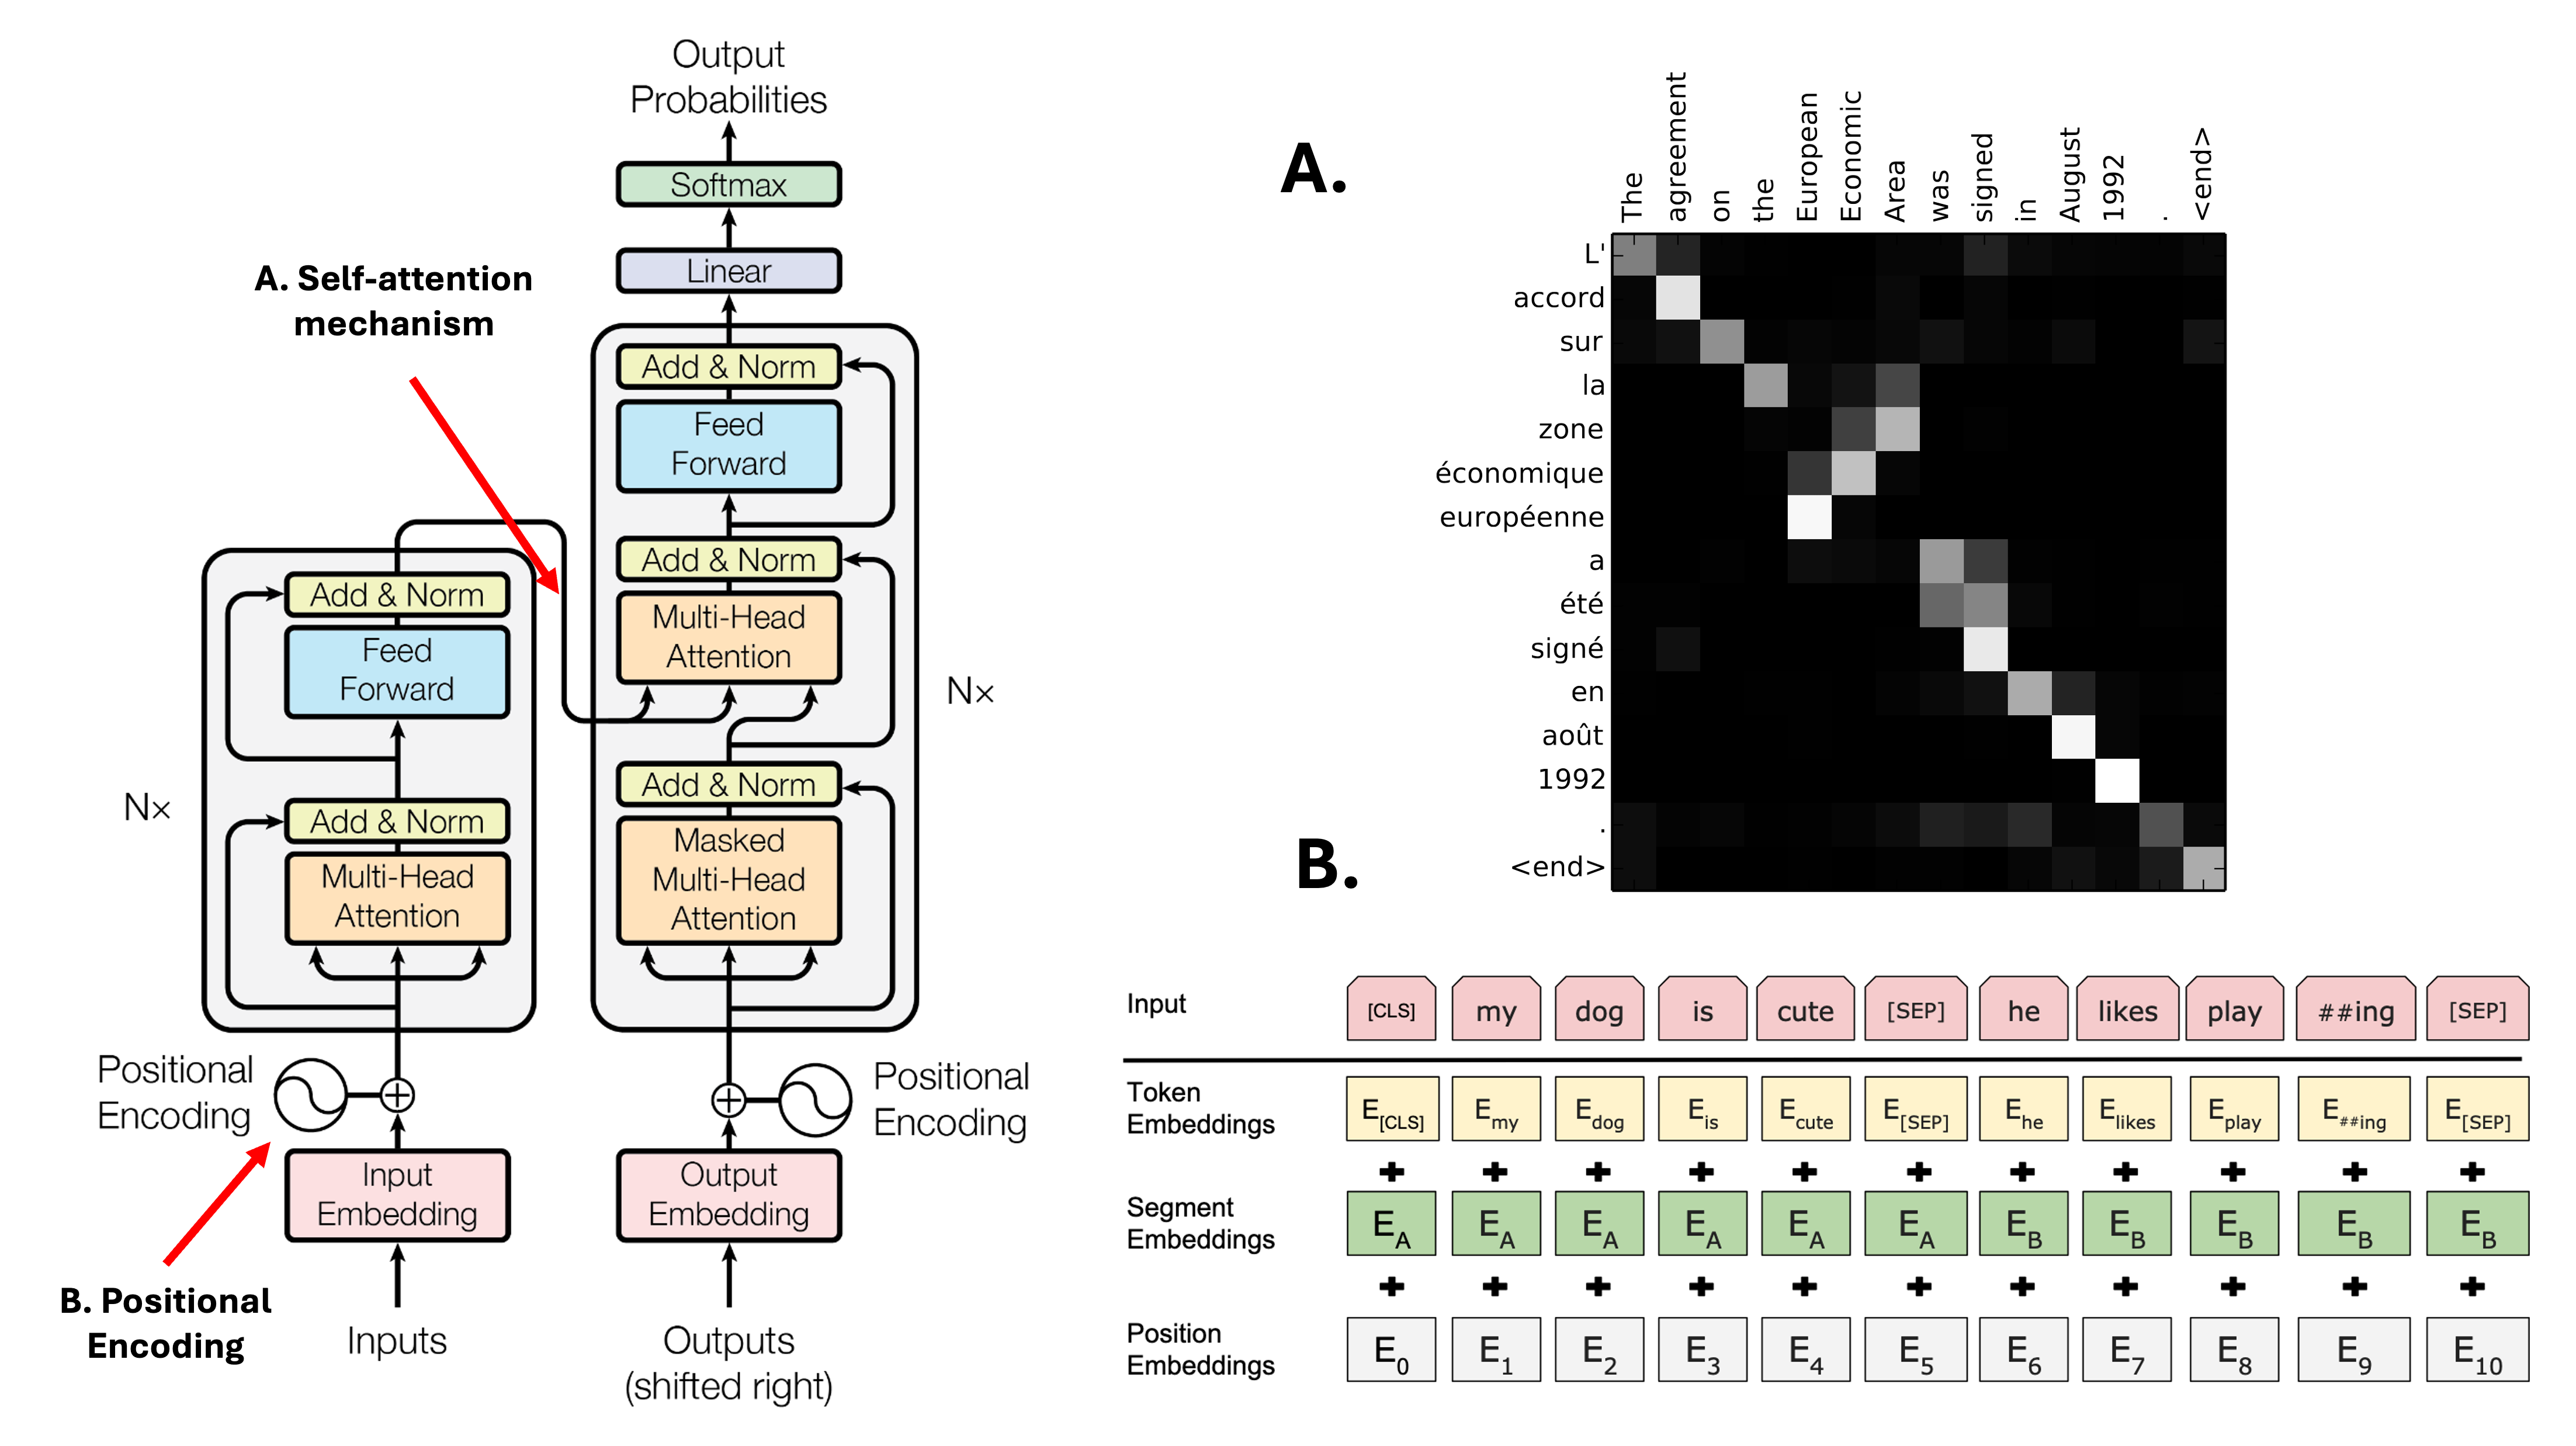
\includegraphics[width=1\linewidth] {figures/transformer_arch.png}
	\caption{Transformer architecture with examples of (A) self-attention and (B) position embeddings \emph{Repurposed from  \cite{NIPS2017_3f5ee243, bahdanauNeuralMachineTranslation2015, devlin-etal-2019-bert}}} \label{fig:transformer}
\end{figure}

Given the sequential nature of human reading comprehension, several model architectures were developed that employed neural networks to model text sequences (i.e. RNNs, LSTMs) \citep{jozefowicz2016exploring}. However, their slow training times led to the development of more parallelizable architectures. Hence, in 2017, the transformer was developed in the seminal paper entitled "Attention is all you Need" \citep{NIPS2017_3f5ee243}. This model has two main features that differentiate it from all prior neural network architectures: positional embeddings and attention. As shown in Figure~\ref{fig:transformer}A, attention allows the transformer to learn based on the entire sentence, rather than just the preceding text, like in RNNs. 

Eventually, the general-purpose transformer architecture was extended to explicitly learn distributional semantics through BERT \cite{devlin-etal-2019-bert} and GPT \cite{radford2018improving}. BERT models only used the encoder component of the transformer architecture, while GPT models only used the decoder component. Because sequence is not explicitly encoded within transformers, it must be introduced elsewhere to ensure that the order of words is remembered. This is done with position encoding as in Figure~\ref{fig:transformer}B, in which a position embedding, along with the segment and token embeddings, define the word embedding within transformer-based models. One final improvement from the original word2vec models was developed to resolve their inability to handle out-of-vocabulary (OOV) words. As word2vec models used human-readable words, scaling them to human language would require an intractable number of words. Instead, tokenization schemes at the subword (similar to morphemes, but statistically driven) level, such as byte-pair encoding were developed that naturally compromised some expressivity for full coverage \cite{sennrich-etal-2016-neural}. Interestingly, BERT is trained on a similar training objective as the CBOW model, known as masked language modeling, where a word is hidden and the model is trained to reproduce it. Unlike BERT, GPT models are trained on next word prediction, similar to the original RNN-based models. These models revolutionized modern-day NLP and distributional semantics models. 

These initial models had an incredible number of trainable parameters ($BERT_{Base}$: 110M, $BERT_{Large}$: 340M). However, it was soon found that performance and expressiveness increase with scale, and as a function of scale, compute \cite{kaplan2020scaling, bahriExplainingNeuralScaling}, leading to current sizes of 70B parameters in open models. They're huge sizes have earned then the name Large Language Models (LLMs). In addition to the increased performance, these models have also progressively increased their context windows, now able to handle up to 128K tokens, allowing them to take even larger sections of text into context in both training word embeddings and in prediction \cite{openaiGPT4TechnicalReport2024}. We believe that this unique set of characteristics allow the current state-of-the-art LLMs to model sublanguage grammars effectively.

\subsection{Distributional semantic models as fuzzy sub-language grammars}
The main limitation that we've seen thus far from the existing clinical sublanguage grammar is its inability to handle anaphora detection due to single-sentence structures. However, the aforementioned large context windows and self-attention mechanism of modern large language models enable them to identify between-sentence relationships. However, these models come with their own set of limitations, leading to a fuzzy sublanguage grammar. As we have discussed, a sublanguage grammar requires two main components (in addition to abiding by the rules of the larger English grammar): word classes, and relationships between word classes as sentence structures. However, distributional semantic models such as large language models do not operate on the word level to begin with. Instead, as we discussed, most use subword encoding schemes such as byte-pair encoding. Therefore, unless they are able to demonstrate co-occurrence recognition at the word level, they cannot be considered sublanguage grammars. This also has consequences for their efficacy in word-level downstream tasks. Therefore, a line of work has investigated if more knowledge-based, clinically meaningful tokenization schemes would significantly improve results. For instance, \citet{jimenezgutierrezBiomedicalLanguageModels2023} find that pretraining BERT-based models on segmented morpheme data cross-referenced with concepts in UMLS does not significantly improve either the pretraining performance of masked language modeling (MLM) nor does it improve results on word-level downstream tasks, such as entity linking and named entity recognition (NER). Additional evidence of subword tokenizers' ability to parse clinical language at the word level comes from French, where only 25\% of downstream tasks including NER and part-of-speech tagging were improved by clinical morpheme-enriched tokenizers \citet{labrak-etal-2024-important}. However, some improvements have been seen \citet{hasanInfusingClinicalKnowledge2024}, leading to the conclusion that current subword tokenization schemes enable large language models to estimate semantic word-classes from subwords, although explicit morpheme-based tokenization would explicitly model the semantics of the clinical sublanguage better at the cost of less lexical coverage. The absence of the word as the most reduced semantic unit in large language models introduces the first element of fuzziness when compared to a strict sublanguage grammar.

In addition to the lack of explicit clinical morphemes in large language models, the word classes themselves, as well as the sentence structures are both also not explicit, leading to a further relaxation of Harris' sublanguage grammar requirements. While large language models do not explicitly model semantic word-classes in a sublanguage grammar, they can be considered leaky abstraction based on co-occurrence matrices. The next-word prediction and MLM pretraining tasks introduce an inductive bias for generating contextual word representations, including varying word senses across different contexts \cite{ethayarajh-2019-contextual}. Notably, sublanguage grammar word classes are often defined by co-occurrences, making this a reasonable model for capturing features of the sublanguage. Another way of validating the claim of strong biases towards word classes in a sublanguage is by looking for irrelevant information. In the fact verification literature, \citet{min-etal-2023-factscore} find that instruction-tuned models, such as InstructGPT and ChatGPT, rarely ($\leq 1.8\%$) generate information irrelevant to the prompt. This is perhaps a function of their RLHF fine-tuning, in which such generation would be heavily non-humanistic and therefore penalized. For our purposes though, while it is possible for them to generate words outside of the semantic classes in the sublanguage, it is highly unlikely. 

The last element of fuzziness in LLMs that may break a formal sublanguage grammar definition would be their lack of explicit accepted sentence structures. While sublanguage grammars are rigid and comprehensive, their parsing can introduce ambiguity. For instance, garden path sentences (a classic example is \emph{Time flies like an arrow; fruit flies like a banana}) are sentences where the expected parse does not align with the syntactically correct parse tree. Another source of ambiguity is abbreviation disambiguation. One can imagine the following sentence within the clinical sublanguage of the sentence structure $Finding + v_{show} + change$: 

\begin{quote}
\emph{Patient's LFTs are trending downwards, which could suggest improvement; will continue monitoring to confirm  stabilization.}
\end{quote}

Without additional context, \emph{LFT} could be confused for either lung function test or liver function test, significantly differentiating the underlying pathology. Both would fit within the aforementioned sublanguage sentence structure as a $Finding$ but have different semantic meaning. Given the already ambiguous nature of parsing sublanguage grammars, large language models introduce additional ambiguity by not formally modeling these grammars. However, work in machine translation to code has shown that LLMs are also capable of translating natural language to domain-specific languages (DSLs) \cite{shin-etal-2021-constrained, wangGrammarPromptingDomainspecific2024}. Therefore, we are confident that these models can effectively capture contextual word-class relationships within sublanguage grammars, even without the grammar being explicitly encoded. Having demonstrated that word classes and syntactic sentence structures can be represented, albeit not formally, by large language models, we are reasonably confident that state-of-the-art models can generate text proficiently within the clinical sublanguage. However, in this thesis, our goal is not only to generate text in the clinical sublanguage but also to investigate how cognitive reasoning aligns between humans and LLMs under conditions of uncertainty in decision-making. Therefore, we next discuss how a normative cognitive framework, combined with the contextual biases of LLMs, can be used to investigate uncertainty-driven clinical reasoning as it relates to physicians.

% Documents in the sublanguage of clinical reporting are distinguished syntactically in various respects. Most striking is that the document "sentences" are often not complete sentences at all. The sentential unit, i. e. the stretch between end-of-sentence punctuation marks, may indeed be a full assertion (The gram stain was negtive); it may also consist solely of a noun phrase (No contact with known infection), a subject + predicate (conjunctivae clear), an assertion lacking only a subject (will be followed in clinic), or certain other forms as illustrated in Fig. 14. It -> From Automatic Information Fomatting of Med sublanguage by Sager


\section{An LLM as a Participant in a Cognitive Clinical Study of Uncertainty}
So far, we have argued that the normative approach affords us certain benefits when using the LLM as a cognitive study participant, such as viewing the LLM as a subexpert physician and evaluating the LLM under a standardized ground truth. We have also validated that the LLM is able to generate text within the clinical sublanguage. Therefore, we must motivate the purpose of investigating its ability to align to a normative approach to diagnostic reasoning through the clinical sublanguage. We argue that there are both technical and sociotechnical reasons for doing so. 

Firstly, as discussed, uncertainty is an inherent part of the clinical decision making process, particularly in diagnosis. In a real-world clinical context, it is impossible to have 100\% certainty before making a diagnosis and further management. Instead, the art of medicine is to weigh the relative risks while gathering more information. As it is unlikely that LLMs will be used with no oversight, they will often function as triggers for further manual review. As such, the weighing of relative risks by the LLM must be better characterized. As we will see in Chapter~\ref{chapter:related-work}, while LLMs have been demonstrated to quantify uncertainty effectively in medical challenge questions (i.e. USMLE question-answering), these are not representative of real-world tasks that physicians and AI will collaborate on. Therefore, our first experiment in Ch.~\ref{chapter:deprescribing} is designed around such a task in which the benefit of discontinuing medications is weighed against the potential cost of adverse withdrawal reactions or return of a medical condition \cite{reeveBenefitsHarmsDeprescribing2014}. 

Secondly, it has been shown that LLMs perpetuate racial and gender biases in a variety of generative language tasks, including medical education, differential diagnosis and medical plan generation \cite{zackAssessingPotentialGPT42024}, while having been instruction-tuned to limit such biases. Therefore, it is clear that while they will not explicitly respond in a sociodemographically biased manner, they may harbor implicit biases as a function of their training data and procedure. However, this underlying bias has not been evaluated in the estimation of risk. Therefore, in Chapter~\ref{chapter:race-bayes}, we investigate the potential for racial bias in a Bayesian clinical diagnostic frame. This will allow us to determine if LLMs estimate risk variably, in an unexpected way. In particular, we look at estimates of sensitivity/specificity and likelihood ratios. We hope to learn contexts in which LLMs' risk evaluations can be trusted in cases where it cannot, allowing for both better understanding of current model capabilities and providing a path for future standardization.

Thirdly, although much of this risk-weighing may not be included in the clinical note (aside from more recent medical-decision making (MDM) sections and medico-legal clarifications), it is at least evidenced by the decisions that the physician makes. Similarly, while the LLM may "explain" its reasoning, it has been shown that they are surprisingly brittle following their own explanations in subsequent reasoning steps \cite{chenModelsExplainThemselves2024}. As LLMs are used for progressively more complicated tasks such as planning, it would be helpful to determine what influences an LLM's sequence of clinical decisions. Our decision process of choice is diagnosis of chest pain in the Emergency Department. We elect to use the normative approach from cognitive science to establish the "optimal" decision making process and compare the LLM to that. In future work, we hope to conduct a decision analysis of expert physicians to compare against, instead of the simulation study proposed in Chapter \ref{chapter:bn-reasoning}. Such fine-grained evaluations will enable greater confidence in LLMs and identify differences in physician and LLM behavior. Knowing where they differ will allow us to better model physician decision making in LLMs and propose more standardized decision making processes in physicians.

Across these three experiments, we hope to rigorously test LLMs' decision-making capabilities under uncertain clinical situations both as a mechanism of risk quantification as well as its impact on diagnostic narrowing. In the coming Chapter, we will describe the associated progress on uncertainty quantification and Bayesian reasoning in LLMs and how our approach contributes to this literature. 